\documentclass[border=10pt]{standalone}
\usepackage{tikz}
\usetikzlibrary{arrows.meta, positioning, calc, fit, shapes.geometric}
\usepackage{amsmath, amssymb}

% Colors
\definecolor{vblue}{RGB}{90,140,200}
\definecolor{dblue}{RGB}{60,110,180}
\definecolor{lbg}{RGB}{235,242,252}
\definecolor{filmred}{RGB}{200,75,60}
\definecolor{filmor}{RGB}{230,150,50}
\definecolor{gnnblue}{RGB}{170,205,240}
\definecolor{gy}{RGB}{105,105,105}
\definecolor{lgreen}{RGB}{80,170,100}

\begin{document}
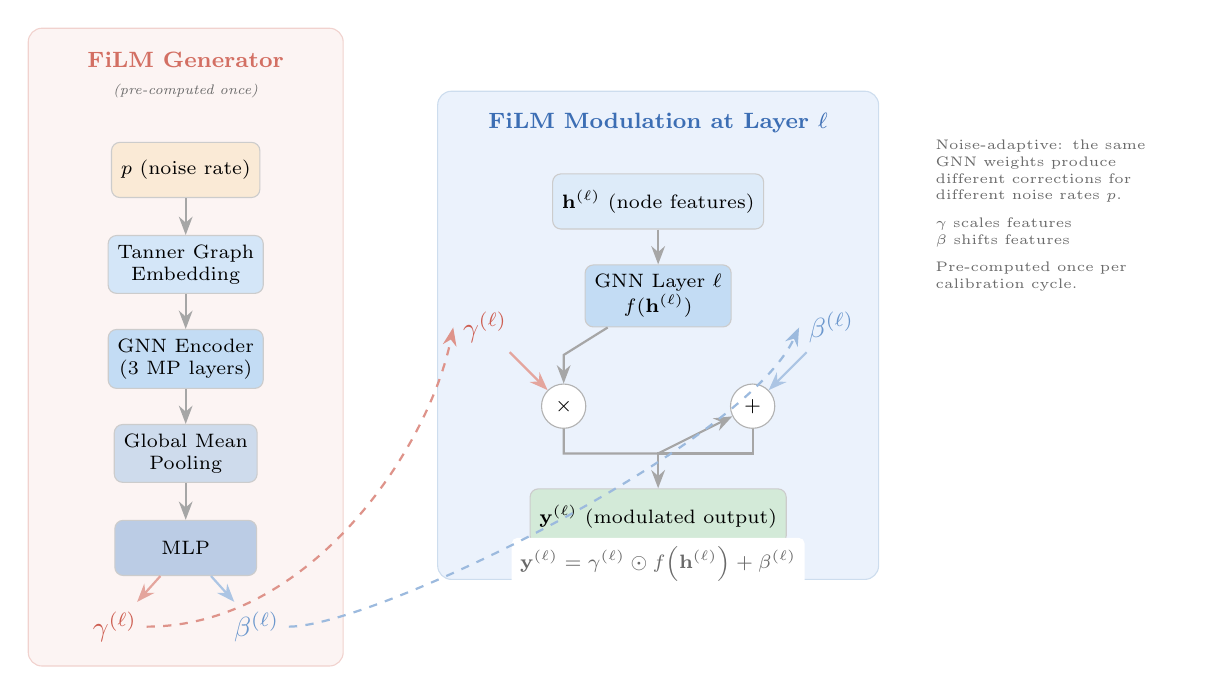
\begin{tikzpicture}[>=Stealth, font=\sffamily,
    block/.style={rectangle, draw=black!20, fill=#1, rounded corners=3pt,
                  minimum width=1.8cm, minimum height=0.7cm,
                  font=\scriptsize, align=center},
    smallblock/.style={rectangle, draw=black!20, fill=#1, rounded corners=2pt,
                       minimum width=1.2cm, minimum height=0.55cm,
                       font=\scriptsize, align=center},
    op/.style={circle, draw=black!30, fill=white, minimum size=16pt,
               font=\scriptsize\bfseries, inner sep=0pt}]

% ════════════════════════════════════════
%  LEFT: FiLM Generator (slow path)
% ════════════════════════════════════════

% Background box
\fill[filmred!6, rounded corners=5pt] (-0.6, -0.3) rectangle (3.4, 7.8);
\draw[filmred!25, rounded corners=5pt] (-0.6, -0.3) rectangle (3.4, 7.8);
\node[font=\footnotesize\bfseries, filmred!80] at (1.4, 7.4) {FiLM Generator};
\node[font=\tiny\itshape, gy] at (1.4, 7.0) {(pre-computed once)};

% Noise parameter input
\node[block=filmor!20] (pval) at (1.4, 6.0) {$p$ (noise rate)};

% Tanner graph embedding
\node[block=gnnblue!50] (tanner) at (1.4, 4.8) {Tanner Graph\\Embedding};

% GNN encoder
\node[block=gnnblue!70] (gnnenc) at (1.4, 3.6) {GNN Encoder\\(3 MP layers)};

% Global pooling
\node[block=dblue!25] (pool) at (1.4, 2.4) {Global Mean\\Pooling};

% MLP
\node[block=dblue!35] (mlp) at (1.4, 1.2) {MLP};

% Outputs
\node[font=\normalsize, filmred!90] (gamma) at (0.5, 0.2) {$\gamma^{(\ell)}$};
\node[font=\normalsize, vblue!90] (beta) at (2.3, 0.2) {$\beta^{(\ell)}$};

% Arrows inside FiLM generator
\draw[->, thick, black!35] (pval) -- (tanner);
\draw[->, thick, black!35] (tanner) -- (gnnenc);
\draw[->, thick, black!35] (gnnenc) -- (pool);
\draw[->, thick, black!35] (pool) -- (mlp);
\draw[->, thick, filmred!50] (mlp) -- (gamma);
\draw[->, thick, vblue!50] (mlp) -- (beta);

% ════════════════════════════════════════
%  CENTER: FiLM Modulation (the key idea)
% ════════════════════════════════════════

% Background box
\fill[lbg, rounded corners=5pt] (4.6, 0.8) rectangle (10.2, 7.0);
\draw[vblue!30, rounded corners=5pt] (4.6, 0.8) rectangle (10.2, 7.0);
\node[font=\footnotesize\bfseries, dblue] at (7.4, 6.6) {FiLM Modulation at Layer $\ell$};

% Input features
\node[block=gnnblue!40] (xin) at (7.4, 5.6) {$\mathbf{h}^{(\ell)}$ (node features)};

% GNN layer
\node[block=gnnblue!70] (gnnlayer) at (7.4, 4.4) {GNN Layer $\ell$\\$f(\mathbf{h}^{(\ell)})$};

% Multiply operator
\node[op] (mul) at (6.2, 3.0) {$\times$};

% Add operator
\node[op] (add) at (8.6, 3.0) {$+$};

% gamma and beta arriving
\node[font=\normalsize, filmred!90] (g_in) at (5.2, 4.0) {$\gamma^{(\ell)}$};
\node[font=\normalsize, vblue!90] (b_in) at (9.6, 4.0) {$\beta^{(\ell)}$};

% Output
\node[block=lgreen!25] (yout) at (7.4, 1.6) {$\mathbf{y}^{(\ell)}$ (modulated output)};

% Flow arrows
\draw[->, thick, black!35] (xin) -- (gnnlayer);
\draw[->, thick, black!35] (gnnlayer) -- (6.2, 3.65) -- (mul);
\draw[->, thick, filmred!50] (g_in) -- (mul);
\draw[->, thick, black!35] (mul) -- (6.2, 2.4) -- (7.4, 2.4) -- (add);
\draw[->, thick, vblue!50] (b_in) -- (add);
\draw[->, thick, black!35] (add) -- (8.6, 2.4) -- (7.4, 2.4) -- (yout);

% The equation
\node[font=\scriptsize, gy, fill=white, inner sep=3pt, rounded corners=2pt]
    at (7.4, 1.0)
    {$\mathbf{y}^{(\ell)} = \gamma^{(\ell)} \odot f\!\left(\mathbf{h}^{(\ell)}\right) + \beta^{(\ell)}$};

% ════════════════════════════════════════
%  Dashed arrows from FiLM generator to modulation
% ════════════════════════════════════════

\draw[->, dashed, filmred!60, thick]
    (gamma.east) .. controls (3.0, 0.2) and (4.5, 2.5) .. (g_in.west);
\draw[->, dashed, vblue!60, thick]
    (beta.east) .. controls (3.8, 0.2) and (8.5, 2.5) .. (b_in.west);

% ════════════════════════════════════════
%  RIGHT: Why FiLM? (annotation)
% ════════════════════════════════════════

\node[font=\tiny, gy, align=left, anchor=north west, text width=3.2cm]
    at (10.8, 6.5)
    {Noise-adaptive: the same\\
     GNN weights produce\\
     different corrections for\\
     different noise rates $p$.\\[4pt]
     $\gamma$ scales features\\
     $\beta$ shifts features\\[4pt]
     Pre-computed once per\\
     calibration cycle.};

\end{tikzpicture}
\end{document}
